\documentclass{article}\usepackage[]{graphicx}\usepackage[]{color}
% maxwidth is the original width if it is less than linewidth
% otherwise use linewidth (to make sure the graphics do not exceed the margin)
\makeatletter
\def\maxwidth{ %
  \ifdim\Gin@nat@width>\linewidth
    \linewidth
  \else
    \Gin@nat@width
  \fi
}
\makeatother

\definecolor{fgcolor}{rgb}{0.345, 0.345, 0.345}
\newcommand{\hlnum}[1]{\textcolor[rgb]{0.686,0.059,0.569}{#1}}%
\newcommand{\hlstr}[1]{\textcolor[rgb]{0.192,0.494,0.8}{#1}}%
\newcommand{\hlcom}[1]{\textcolor[rgb]{0.678,0.584,0.686}{\textit{#1}}}%
\newcommand{\hlopt}[1]{\textcolor[rgb]{0,0,0}{#1}}%
\newcommand{\hlstd}[1]{\textcolor[rgb]{0.345,0.345,0.345}{#1}}%
\newcommand{\hlkwa}[1]{\textcolor[rgb]{0.161,0.373,0.58}{\textbf{#1}}}%
\newcommand{\hlkwb}[1]{\textcolor[rgb]{0.69,0.353,0.396}{#1}}%
\newcommand{\hlkwc}[1]{\textcolor[rgb]{0.333,0.667,0.333}{#1}}%
\newcommand{\hlkwd}[1]{\textcolor[rgb]{0.737,0.353,0.396}{\textbf{#1}}}%
\let\hlipl\hlkwb

\usepackage{framed}
\makeatletter
\newenvironment{kframe}{%
 \def\at@end@of@kframe{}%
 \ifinner\ifhmode%
  \def\at@end@of@kframe{\end{minipage}}%
  \begin{minipage}{\columnwidth}%
 \fi\fi%
 \def\FrameCommand##1{\hskip\@totalleftmargin \hskip-\fboxsep
 \colorbox{shadecolor}{##1}\hskip-\fboxsep
     % There is no \\@totalrightmargin, so:
     \hskip-\linewidth \hskip-\@totalleftmargin \hskip\columnwidth}%
 \MakeFramed {\advance\hsize-\width
   \@totalleftmargin\z@ \linewidth\hsize
   \@setminipage}}%
 {\par\unskip\endMakeFramed%
 \at@end@of@kframe}
\makeatother

\definecolor{shadecolor}{rgb}{.97, .97, .97}
\definecolor{messagecolor}{rgb}{0, 0, 0}
\definecolor{warningcolor}{rgb}{1, 0, 1}
\definecolor{errorcolor}{rgb}{1, 0, 0}
\newenvironment{knitrout}{}{} % an empty environment to be redefined in TeX

\usepackage{alltt}
\usepackage[margin=0.75in]{geometry}
\usepackage[utf8]{inputenc}
\usepackage[T1]{fontenc}
\usepackage{url}
\usepackage[blocks]{authblk}
\usepackage[]{lineno}
\usepackage[superscript]{cite}
\usepackage{xcite}
\usepackage{array}
\usepackage{booktabs}
\usepackage{tabularx}
\usepackage{multirow}
\usepackage[dvipsnames]{xcolor}
\usepackage[colorlinks=true,urlcolor=darkgray,implicit=false]{hyperref}
\usepackage{cleveref}

% Formatting
\setlength\parindent{0pt}
\setlength{\parskip}{1em}
\usepackage{setspace}
%\doublespacing

% Run texcount on tex-file and write results to a sum-file
\immediate\write18{texcount \jobname.tex -out=\jobname.sum}
% Define macro \wordcount for including the counts
\usepackage{verbatim}
\newcommand\wordcount{\verbatiminput{\jobname.sum}}



\IfFileExists{upquote.sty}{\usepackage{upquote}}{}
\begin{document}

\title{Noninvasive prenatal exome sequencing inefficient for detecting single-gene disorders -- problems and possible solutions}

\author[1,2,*]{Dayne L Filer}
\author[1]{Piotr A Mieczkowski}
\author[1]{Alicia Brandt}
\author[3]{Kelly L Gilmore}
\author[1,2]{Bradford C Powell}
\author[1]{Jonathan S Berg}
\author[1,2,4]{Kirk C Wilhelmsen}
\author[1,3]{Neeta L Vora}
\affil[1]{Department of Genetics, School of Medicine, UNC Chapel Hill, Chapel Hill, NC}
\affil[2]{Renaissance Computing Institute, Chapel Hill, NC}
\affil[3]{Department of Obstetrics \& Gynecology, School of Medicine, UNC Chapel Hill, Chapel Hill, NC}
\affil[4]{Department of Neurology, School of Medicine, UNC Chapel Hill, Chapel Hill, NC}
\affil[*]{Corresponding author: 100 Europa Drive Suite 540, Chapel Hill, NC 27517, \href{mailto:dayne_filer@med.unc.edu}{dayne\_filer@med.unc.edu}}
\date{}

\maketitle

\linenumbers

\section{Bulleted statements}

What's already known about this topic?
\begin{itemize}
    \item Sequencing-based noninvasive testing detects large copy number abnormalities and some single-gene disorders
    \item Fetal exome sequencing (ES) provides 20\% diagnostic yield for structural abnormalities after normal karyotype \& microarray
\end{itemize}

What does this study add?
\begin{itemize}
    \item Cell-free ES in three gravid patients with suspected genetic disease in the fetus
    \item Discussion of probability theory underlying non-invasive fetal genotyping
    \item We demonstrate broad sequencing approaches are limited by sampling and technical difficulties, concluding broad sequencing is currently inappropriate for noninvasive testing
\end{itemize}

\section*{Abstract}

Objective: Sequencing cell-free DNA now allows detection of large chromosomal abnormalities and dominant Mendelian disorders in the prenatal period.
Improving upon these methods would allow newborn screening programs to begin with prenatal genetics, ultimately improving the management of rare genetic disorders.

Methods: As a pilot study, we performed exome sequencing on the cell-free DNA from three mothers with singleton pregnancies to assess the viability of broad sequencing modalities in a noninvasive prenatal setting.

Results: We found poor resolution of maternal and fetal genotypes due to both sampling and technical issues.

Conclusion: We find broad sequencing modalities inefficient for noninvasive prenatal applications.
Alternatively, we suggest a more targeted path forward for noninvasive prenatal genotyping.

\section{Introduction}

The beneficial health outcomes from newborn screening programs (NBS) are indisputable.
We envision future NBS will begin with prenatal genetic testing to enable care in the immediate newborn period, and open up new possibilities for \textit{in utero} and genetic therapies.
During pregnancy, placental DNA is released into maternal circulation, enabling noninvasive interrogation of fetal genetics (noninvasive prenatal testing, NIPT).
NIPT has a well-established clinical utility in screening for common chromosomal abnormalities such as Down syndrome with high sensitivity and specificity\cite{mackie:2017aa}.
More recently, efforts have demonstrated sequencing-based testing for \textit{de novo} pathogenic variants in a list of 30 genes associated with dominant Mendelian disorders \cite{zhang:2019aa} and PCR-based testing for a small number of recessive Mendelian disorders \cite{tsao:2019ab}.
Using relative haplotype dosage analysis (RHDO) \cite{lo:2010aa}, multiple groups have successfully diagnosed single gene disorders \cite{hui:2017aa,vermeulen:2017aa,jang:2018aa} including a new offering of noninvasive prenatal diagnosis for cystic fibrosis in the UK Public Health Service \cite{chandler:2020aa}.
RHDO typically relies on collecting parental, and ideally proband, genetic information to resolve parental haplotypes; Jang et al. demonstrated success in diagnosing Duchenne muscular dystrophy by estimating haplotypes solely from maternal long-read sequencing \cite{jang:2018aa}.
Scotchman et al. provide an excellent review summarizing the history of noninvasive testing \cite{scotchman:2020aa}.
To date, no one has reported reliable fetal genotyping purely from maternal cell-free DNA using a sequencing-based approach.

To begin NBS with prenatal genetic testing, we believe we first need a reliable noninvasive test only requiring a maternal sample.
Others could reasonably argue the availability of carrier screening, and the immeasurably small risk of invasive testing \cite{salomon:2019aa}, removes the need for noninvasive testing.
Such an argument, however, dismisses (1) the ethical and practical issues surrounding the necessity of involving the biological father, (2) the fact that many genetic disorders arise due to \textit{de novo} mutations, and (3) the understandable fear and apprehension around invasive testing (especially for rare conditions).
Additionally, we believe the prenatal diagnosis community should focus work on sequencing-based (as opposed to PCR-based) approaches.
Sequencing generalizes across disorders more easily than PCR techniques, allows multiplexing to a degree not feasible using PCR, and will only continue to decrease in cost.

Snyder et al. provide a review of previous attempts to perform noninvasive fetal genome sequencing, illustrating the cost-infeasibility and suggesting more targeted approaches such as exome sequencing (ES) \cite{snyder:2013aa,lo:2010aa,kitzman:2012aa,fan:2012aa}.
As an exploratory exercise, we performed ES on cell-free DNA (cfES) from three pregnant women with singleton fetuses.

\section{Methods}

\subsection{Participant selection}
Genetic counselors identified pregnant women with suspected genetic disorders based either on family history or fetal sonographic findings.
We enrolled three women, blinded to their family history and sonographic findings.
All participants were consented and enrolled at UNC Hospitals by certified genetic counselors with approval from the UNC Institutional Review Board (IRB Number: 18-2618); we do not include any identifying information in this manuscript.

\subsection{Exome sequencing and analysis}
We collected cell-free DNA from maternal plasma, prepared sequencing libraries for the Illumina platform, and performed exome capture using the IDT xGen Exome Research Panel v1.0 (Cases 1 \& 2) or Agilent SureSelect Human All Exon v7 (Case 3).
We processed the data using a novel analytic pipeline developed in Snakemake \cite{koster:2012aa} using Anaconda environments for reproducibility (provided in supplemental materials).
Briefly, sequencing reads were aligned to hg38 (excluding alternate contigs) using BWA-MEM \cite{li:2013ab}, then base quality scores were re-calibrated using GATK4 \cite{mckenna:2010aa,van-der-auwera:2013aa,poplin:2018aa}.
We only retained non-duplicate, properly-paired reads with unambiguous mapping and mapping quality >30 for each read.
We called variants using bcftools \cite{li:2011aa}, requiring basepair quality scores >20.
We suggest the review by Seaby et al. for more information on the specifics of collecting and processing ES data for clinical use \cite{seaby:2016aa}.
Analyses were restricted to the regions overlapping between the IDT and Agilent capture platforms.
For cell-free analyses, we required 5 alternate allele-supporting read-pairs, and at least 80 total read-pairs.
Using the identified single-nucleotide variants, we applied a novel empirical Bayesian procedure to estimate the fetal fraction (FF; the proportion of placental/fetal to maternal sequencing reads).
We then estimated maternal and fetal genotypes using a maximal likelihood model incorporating the FF estimate and observed proportion of minor allele (alternate) reads (PMAR).
The full details of the algorithm are provided in supplemental materials, including an R \cite{r-core-team:2019aa} package reproducing our results for complete transparency: \url{https://github.com/daynefiler/filer2020B}.

\subsection{Data availability}
The data that support the findings of this study are available on request from the corresponding author.
The raw sequencing data are not publicly available due to privacy or ethical restrictions.
Allele depths, with the alleles masked and genomic location rounded to 10 kilobases are available in the self-contained R package reproducing the analysis herein (\url{https://github.com/daynefiler/filer2020B}).

\section{Results}

\begin{table}
  \centering
  \begin{tabular}[t]{
  >{\raggedright}p{\dimexpr 0.03\linewidth-2\tabcolsep-1.125\arrayrulewidth\relax}
  >{\raggedright}p{\dimexpr 0.09\linewidth-2\tabcolsep-1.125\arrayrulewidth\relax}
  >{\raggedright}p{\dimexpr 0.26\linewidth-2\tabcolsep-1.125\arrayrulewidth\relax}
  >{\raggedright}p{\dimexpr 0.26\linewidth-2\tabcolsep-1.125\arrayrulewidth\relax}
  >{\raggedright}p{\dimexpr 0.09\linewidth-2\tabcolsep-1.125\arrayrulewidth\relax}
  >{\raggedright}p{\dimexpr 0.09\linewidth-2\tabcolsep-1.125\arrayrulewidth\relax}
  >{\raggedright}p{\dimexpr 0.09\linewidth-2\tabcolsep-1.125\arrayrulewidth\relax}
  >{\raggedright\arraybackslash}p{\dimexpr 0.09\linewidth-2\tabcolsep-1.125\arrayrulewidth\relax}
  }
  \toprule
   & GA & Clinical findings & Genetic diagnosis & FF & Depth & \%Dup & \%Filt \\
  \midrule
   1 & 32w2d & 5 prior pregnancies affected with X-linked recessive Menke's syndrome & Menke's syndrome; del. ATP7A exon 1 & 0.117 & 241 & 42.8 & 21.96 \\
   2 & 24w5d & Fetal sonogram at 21w5d showed femoral bowing with shortened length (<3\% for GA) bilaterally & Osteogenesis imperfecta type VIII; P3H1 c.1120G>T (rs140468248) & 0.122 & 152 & 33.32 & 22.09 \\
   3 & 34w0d & Fetal sonogram at 19w0d showed bilateral club foot with bilateral upper limb arthrogryposis & None, to date, despite exome and genome sequencing of newborn & 0.169 & 330 & 53.67 & 32.65 \\
  \bottomrule
  \end{tabular}
  \caption{Case summaries. GA: gestational age at the time of blood draw for cfES. FF: estimated fetal fraction. Depth: median depth used to estimate genotypes (does not include duplicated/filtered reads). \%Dup: percentage of total mapped read pairs discarded as PCR and/or optical duplicates. \%Filt: percentage of total mapped read pairs discarded for improper pairing and/or mapping quality.}
  \label{tab:cases}
\end{table}

Using the final set of filtered reads, we analyzed single nucleotide loci with >80x coverage and at least 5 reads supporting the alternate allele.
At each analyzed site, we alternate allele sequencing depth and total sequencing depth to estimate the fetal fraction and maternal-fetal genotypes using our novel algorithm (\cref{fig:genoHist}).
\Cref{tab:cases} lists the known genetic diagnoses for the three cases presented.
Genetic counselors recruited the three participants; investigators and cfES analysis was blinded to the eventual genetic diagnoses.
In Cases 1 \& 2, specific gene sequencing based on family history and sonographic findings, respectively, provided genetic diagnoses.
To date, Case 3 does not have a genetic diagnosis.
We learned the mother in Case 1 carries a deletion of exon 1 in the gene most-often responsible for Menke’s syndrome (ATP7A).
Neither exome capture platform targets ATP7A exon 1; therefore, cfES could not have identified the diagnosis for Case 1 with the platform used.
In Case 2, we identified the causal variant using cfES.
In this case, we correctly genotyped the fetus, but lacked the power to make the genotyping call with any level of confidence acceptable for clinical use (\cref{fig:genoHist}B, note the widely-overlapping distributions at the causal variant).
We did not identify any known pathogenic variants in the sequencing of Case 3, and despite performing genome sequencing on the newborn, we still do not have a genetic diagnosis for the family.

In Case 3, in addition to cfES, we performed exome sequencing (ES) on fetal, maternal, and paternal samples.
Based on previous work demonstrating the differential length of maternal and fetal fragments \cite{chan:2004aa,chan:2016aa,jiang:2016ab,rabinowitz:2019aa}, we interrogated the distribution of presumed maternal and fetal reads (\cref{fig:c3fragLen}).
We identified maternal and fetal reads by identifying sites with unique heterozygosity in the direct maternal and fetal ES results; at the informative sites, we extracted reads supporting the allele unique to the mother or fetus.
In total, we identified 654,619 maternal reads and 279,508 fetal reads.
We found, as others have, a higher proportion of fetal reads falling below 150 basepairs; however, we also observed a slightly higher proportion of longer reads, as well.

Rabinowitz et al. proposed the Hoobari method which incorporates fragment lengths into fetal genotype estimates \cite{rabinowitz:2019aa}, finding the difference in accuracy varied from -0.25\% to 1.89\% when using versus not using fragment length in their exome analyses.
To explore the utility of correcting for fragment length in our analysis, we interrogated the PMAR as a function of the short read proportion (fraction of reads with insert sizes less than 140 basepairs; \cref{fig:pmarBySratio}).
We selected 140 as the cutoff based on the Hoobari algorithm.
Overall, we found no meaningful relationship between the short read proportion and the observed PMAR and chose not to incorporate fragment length into our genotype estimates.

Returning to Case 3, we interrogated the fetal genotyping accuracy at all sites with cell-free genotype estimates and reliable calls from the direct fetal sample.
Overall, we found a 50.91\% accuracy (\cref{tab:c3calls}).
We provide the complete set of calls within the R package, and a summary within the supplemental document.

\begin{table}
  \centering
  \begin{tabular}{llrrr}
  \toprule
   & & \multicolumn{3}{c}{Cell-free} \\
   & & aa & ab & bb \\
   \midrule
   \multirow{3}{*}{Fetal} & aa & 1063 & 1857 & 9 \\
   & ab & 3598 & 7079 & 1454 \\
   & bb & 76 & 2197 & 1391 \\
  \bottomrule
  \end{tabular}
  \caption{Case 3 fetal versus cell-free calls. 'a' represents the major allele; 'b' represents the minor allele. Sites with cell-free estimates and reliable direct fetal calls included (reliable defied as passing all quality checks and having a total sequencing depth greater than 30).}
  \label{tab:c3calls}
\end{table}

\begin{figure}
  \centering
  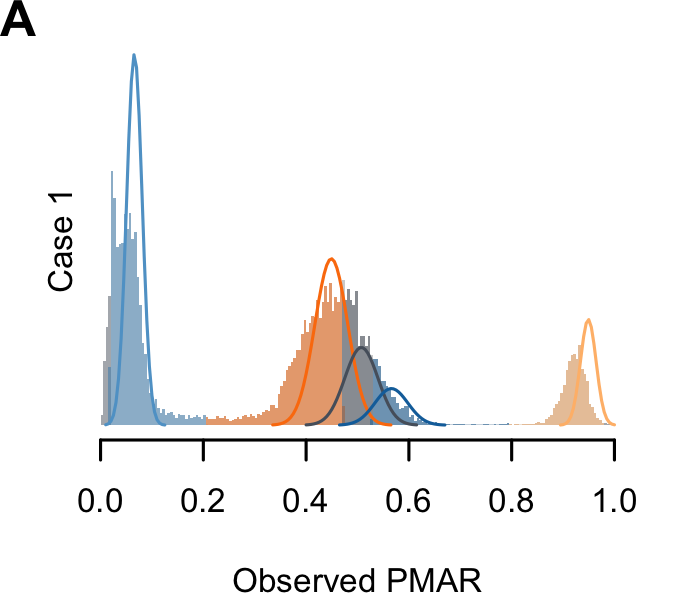
\includegraphics{fig-genoHist-1.pdf}%
  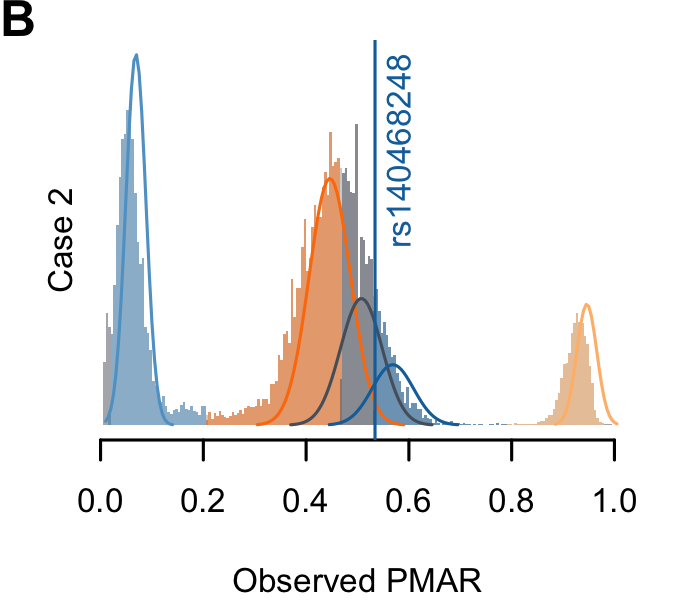
\includegraphics{fig-genoHist-2.pdf}%
  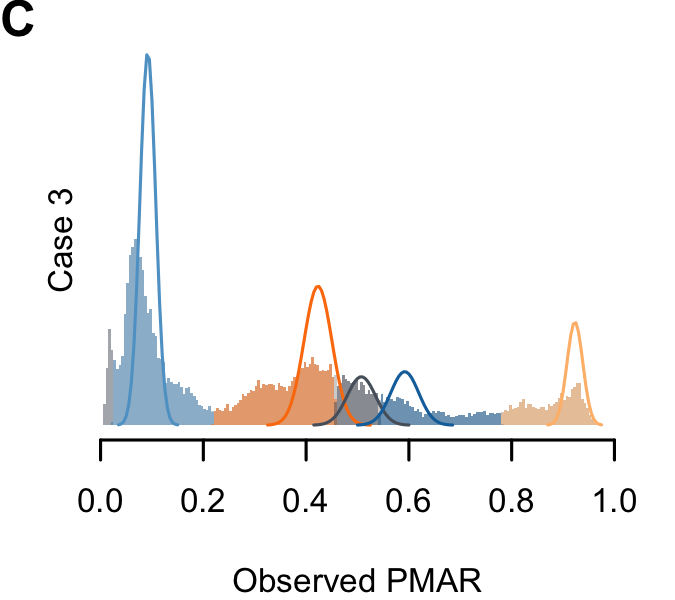
\includegraphics{fig-genoHist-3.pdf}
  
\includegraphics{fig-genoLgnd-1.pdf}
  \caption{Distribution of observed proportion of minor allele reads (PMAR) values for the three cases across the possible maternal-fetal genotype pairs. Uppercase letters give the estimated maternal genotype, lowercase letters give the estimated fetal genotype; `A/a' indicates the reference allele, `B/b' indicates the alternate allele. Solid lines show the normal approximation for the theoretical distribution of binomial probabilities, given the frequency of the estimated genotypes. The vertical line in [B] shows the observed PMAR for the known pathogenic variant, rs140468248.}
  \label{fig:genoHist}
\end{figure}

\begin{figure}
  \centering
  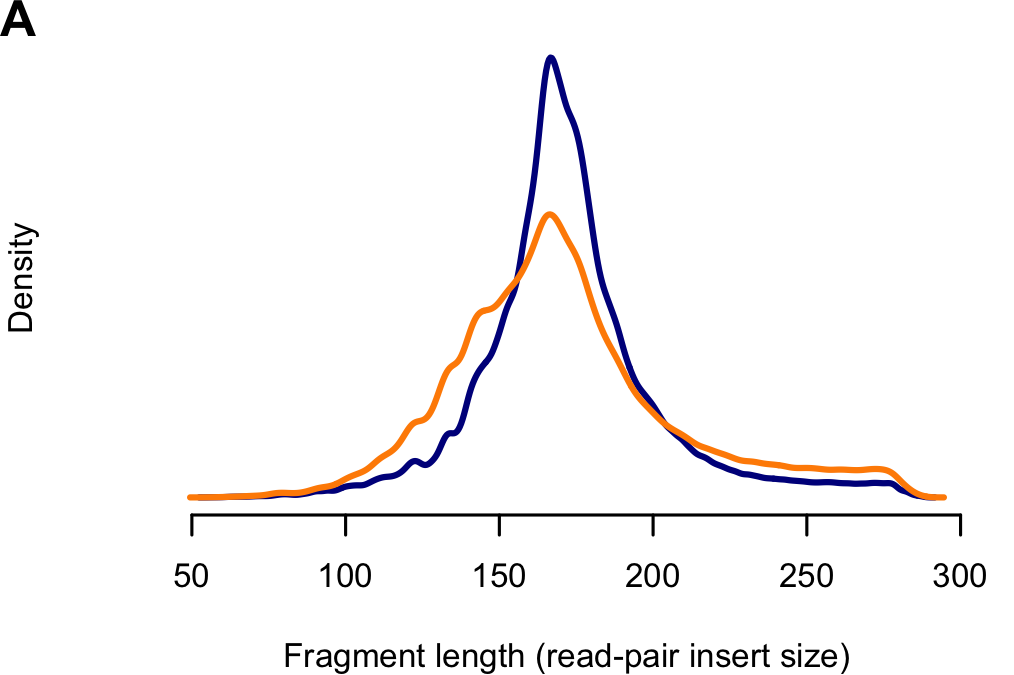
\includegraphics{fig-f34FragLen-1.pdf}%
  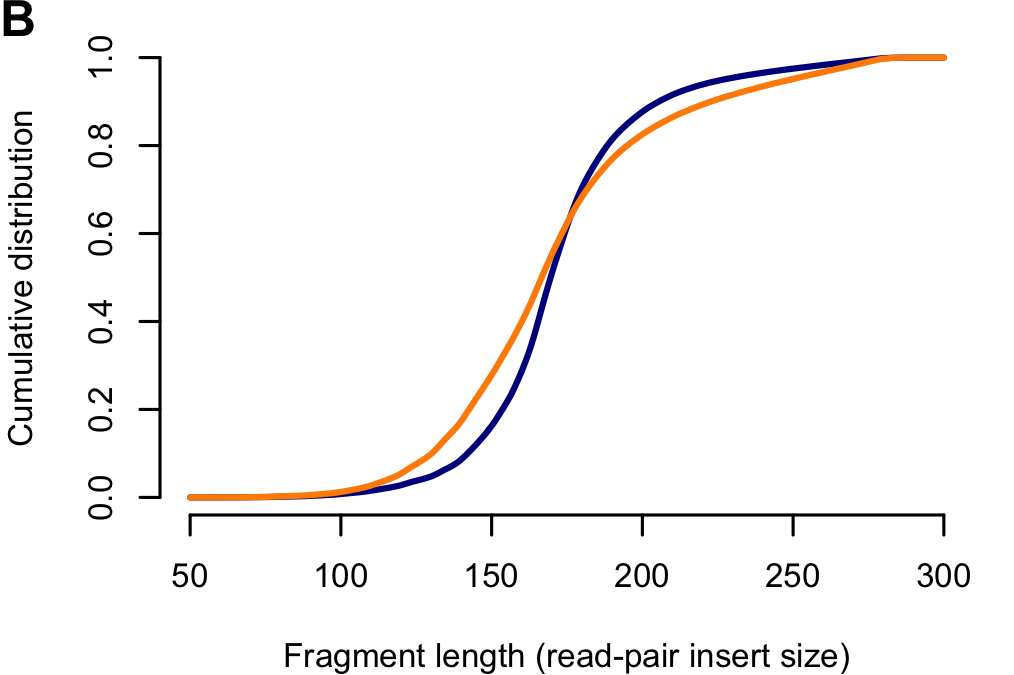
\includegraphics{fig-f34FragLen-2.pdf}
  
\includegraphics{fig-fragLgnd-1.pdf}
  \caption{Distribution of maternal versus fetal fragment length in Case 3. [A] shows the density; [B] shows the emperic cumulative distribution. The horiztonal axis shows the fragment length (insert size taken from aligned read-pairs). Blue lines show maternal reads, orange lines show fetal reads. We only included cfES reads supporting alleles unique to the mother or fetus, as identified from the direct maternal and fetal ES.}
  \label{fig:c3fragLen}
\end{figure}

\begin{figure}
  \centering
  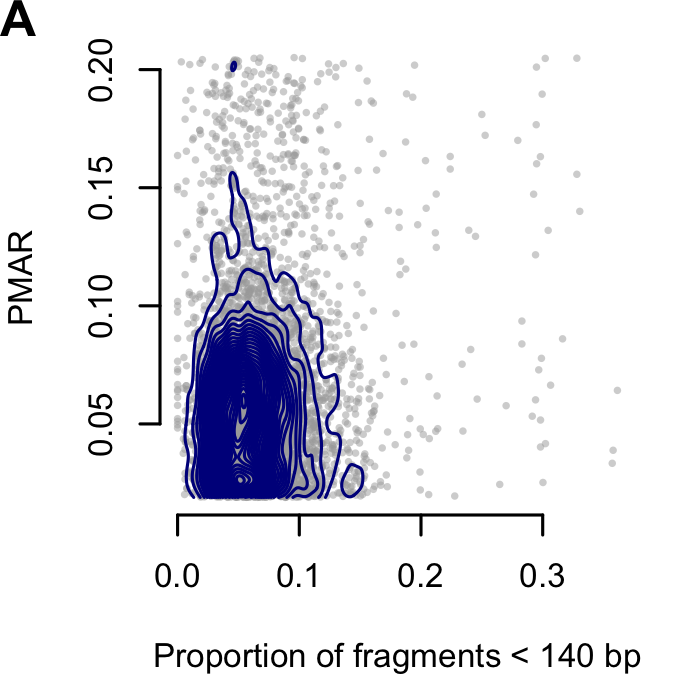
\includegraphics{fig-pmarBySratio-1.pdf}%
  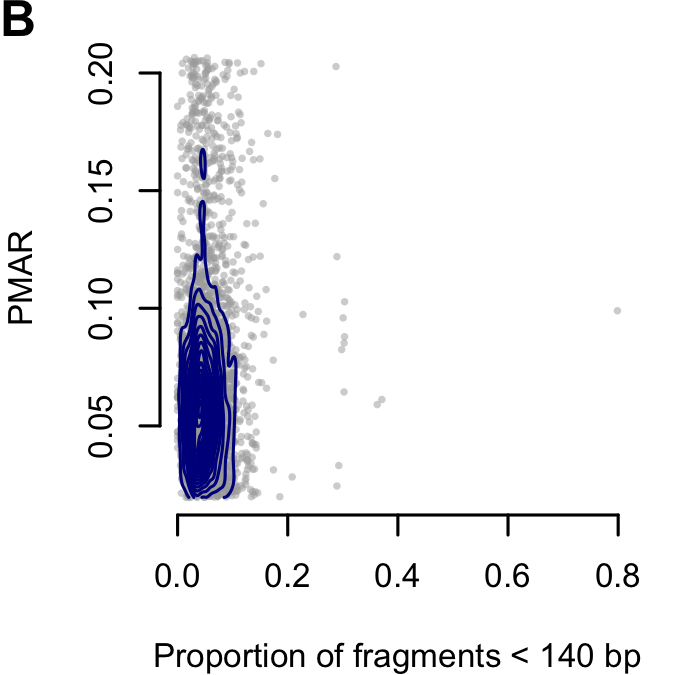
\includegraphics{fig-pmarBySratio-2.pdf}%
  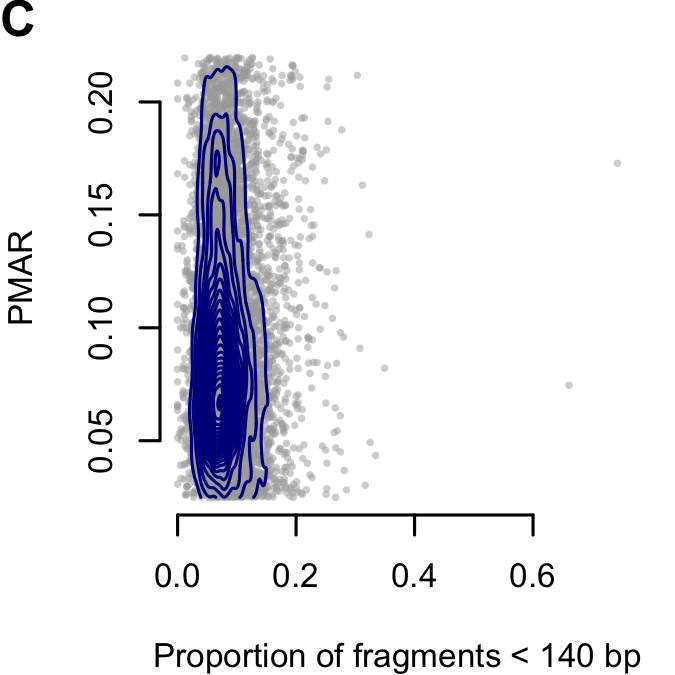
\includegraphics{fig-pmarBySratio-3.pdf}
  \caption{Proportion of minor allele reads (PMAR) as a funciton of the short read proprtion for genotypes estimated as `AAab.' Short reads defined as fragments less than 140 basepairs. [A-C] show Cases 1 to 3, respectively. Gray points show the individual sites; blue contour lines show the two-dimensional distribution of values.}
  \label{fig:pmarBySratio}
\end{figure}

\section{Discussion}

Without the ability to reliably exclude maternal DNA fragments, noninvasive sequencing-based methods to genotype the fetus either require additional sequencing of parental samples or distinguishing genotypes by the proportion of minor allele reads (PMAR).
Here, we make no attempt to utilize parental genetic information and demonstrate the difficulty of inferring the genotypes directly from the PMAR.
We model the PMAR as a binomial proportion; given the fetal fraction, one can prove the true PMAR defines the maternal and fetal genotypes (supplemental document).

\begin{figure}
  \centering
  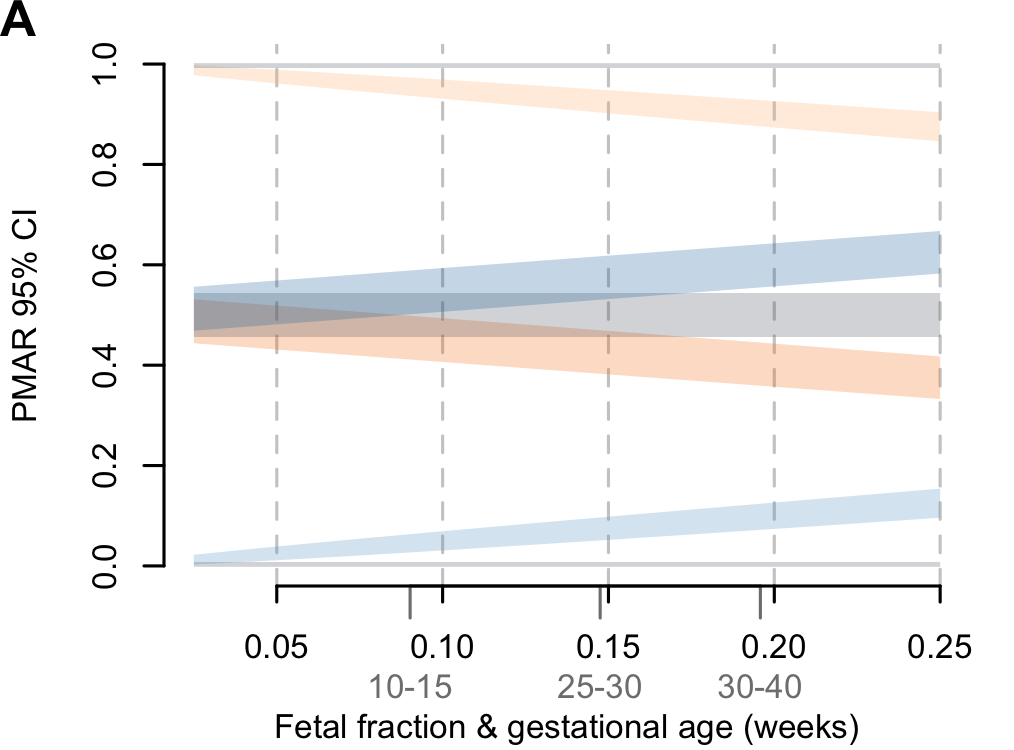
\includegraphics{fig-binDist-1.pdf}%
  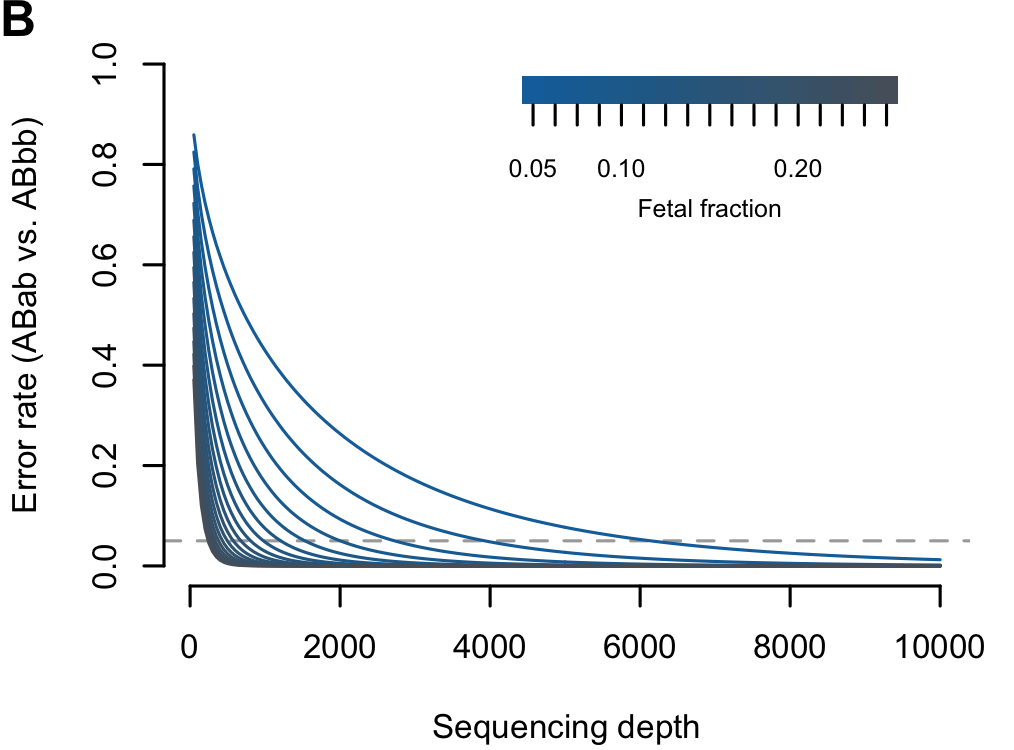
\includegraphics{fig-binDist-2.pdf}
  
\includegraphics{fig-genoLgnd-1.pdf}
  \caption{Binomial distribution limitations. [A] 95\% confidence intervals on the binomial proportions for possible maternal-fetal genotype pairs across increasing fetal fractions; represents a sequencing depth of 500x. Average fetal fractions by gestational age (in weeks) given in light gray \cite{kinnings:2015aa}. [B] Expected misclassification rate (Weitzman overlapping coefficient; i.e. the area of overlapping distributions in [A]) considering ABab versus ABbb as a function of sequencing depth and fetal fraction. The dashed horizontal line shows 5\% error. The theoretical error rates for ABab vs ABaa are symmetric and equal; however, the frequency of errors will depend on the population frequency of the reference versus alternate allele.}
  \label{fig:binDist}
\end{figure}

The theoretical bounds of the binomial distribution, therefore, confine our ability to discriminate maternal-fetal genotypes.
Using the normal approximation for the binomial variance (valid when the number of observations, i.e. sequencing depth, times the binomial proportion, i.e. PMAR, is greater than 10), we can clearly explain the poor results we observed (\cref{fig:binDist}).
At sequencing depths up to 500x, the 95\% confidence intervals on PMAR distributions still overlap for fetal fractions up to roughly 0.17 (\cref{fig:binDist}A).
When we calculate the degree of distribution overlap (a proxy for classification error rate), we see required sequencing depths in excess of 8,000x for low fetal fraction samples (\cref{fig:binDist}B).
We, therefore, cannot expect cell-free sequencing to reliably differentiate genotypes without substantially higher depth or additional genetic information.
No amount of cleverness in the analysis can overcome the fundamental variance bounds when estimating binomial proportions.

The sequencing herein suffers from three problems: (1) inadequate sequencing depth; (2) biased PMAR values from the removal of duplicate reads; (3) errors in sequencing and/or PCR.
We have already illustrated the inadequate depth, but emphasize that the theoretical results we present speak to the final depths (not the raw sequencing depth).
In our three cases, we excluded over half the reads taken off the sequencer due to sequencing quality thresholds (\cref{tab:cases}).
We observe the evidence of problems (2) and (3) by observing the high proportion of both duplicate reads and PMAR values outside the theoretic distributions.
Additionally, we observed very poor accuracy in the Case 3 genotype estimates.

Typical sequencing workflows start with randomly fragmenting DNA molecules to build sequencing libraries.
Standard bioinformatic practices suggest we remove read-pairs with identical endpoints, because the duplicate read-pairs more likely represent PCR amplification of a single molecule than two molecules with the same fragmentation.
Cell-free DNA molecules are shorter than nuclear DNA, not requiring manual fragmentation, and have a non-random distribution of endpoints \cite{chan:2016aa}.
Therefore, compared to standard sequencing libraries, the likelihood of observing true duplicates in cell-free libraries increases and we cannot necessarily assume duplicates represent PCR amplification.
However, for this work we have no way of differentiating reads representing true duplicate molecules versus PCR duplicates and thus excluded duplicate reads from our analysis.

Assuming adequate depth and appropriate handling of duplicate reads and sequencing errors, incorporating the fragment length into the statistical model may prove more beneficial.
The high variability of the binomial distribution for small $n$ obfuscates any meaningful relationship between fragment length and PMAR in our data.
We reiterate, however, incorporating fragment length may give better estimates of the binomial proportion but cannot decrease variance beyond the distribution bounds.

To solve the above issues, we advocate a more targeted approach with much greater sequencing depth and unique molecular identifiers.
Unique molecular identifiers allow identification of sequencing errors and differentiate true versus artifactual duplicate reads.
Given the depth requirements for estimating fetal genotypes by the PMAR, and the challenge of variants of uncertain clinical significance, we advocate against broad sequencing modalities on noninvasive samples.
Recognizing that all capture methods introduce bias in the relative sequencing efficiency of different targeted regions \cite{seaby:2016aa}, the sequencing depths needed for noninvasive fetal genotyping necessitate a targeted approach.
Despite the challenges raised by this work, we believe assessing hundreds to thousands of basepairs, rather than the tens of millions targeted in ES, will prove economical and clinically reliable.
Doing so, we hope, will foster population-level screening for Mendelian disorders during the prenatal period and, ultimately, unlock new avenues in the treatment of these disorders.

\nolinenumbers

\section*{Acknowledgements}
We thank Dr. James Evans for providing review and feedback of this manuscript.
Neeta Vora and this work was supported by NICHD (K23HD088742).
Dayne Filer was supported by NICHD (F30HD101228) and by NIGMS (5T32GM067553).

\bibliographystyle{unsrt}
\bibliography{myBib.bib}

\newpage
\section*{Word count}
\wordcount

\end{document}




